%=====================================================================
%  Advanced Optimization  --  Chapter 12  (12pt edition, v8)
%  Nocedal & Wright, Chapter 12: Theory of Constrained Optimization
%  Organized around what differs from a convex problem:
%  tangent cone and LICQ (12.2), KKT as a necessary condition (12.3),
%  second-order conditions (12.5); then sensitivity (12.8), duality (12.9).
%  The deck is meant to be self-contained: symbols are defined before use.
%
%  Layout rules for this deck (preamble copied from ch07v3.tex)
%   - body 12pt; nothing in the body below 10pt; footline 8pt
%   - one theorem per slide, or at most three displayed equations
%   - proofs are omitted; a red "Read:" pointer gives the pages in the book
%   - equation numbers and theorem statements follow the book
%   - material that is not in the book is marked "(Not in the book.)"
%   - figures are redrawn, not copied from the book
%   - no [shrink] option anywhere
%=====================================================================
\documentclass[aspectratio=169,12pt]{beamer}

\usetheme{default}
\usecolortheme{seahorse}
\useinnertheme{rectangles}
\setbeamersize{text margin left=7mm,text margin right=7mm}
\setbeamertemplate{navigation symbols}{}
\setbeamerfont{title}{series=\bfseries,size=\LARGE}
\setbeamerfont{subtitle}{size=\large}
\setbeamerfont{institute}{size=\small}
\setbeamerfont{frametitle}{series=\bfseries,size=\large}
\setbeamerfont{block title}{series=\bfseries,size=\normalsize}
\setbeamerfont{footline}{size=\scriptsize}   % 8pt at 12pt base
\setbeamercolor{frametitle}{fg=black!85,bg=black!5}
\setbeamercolor{block title}{bg=structure!25,fg=black!85}
\setbeamercolor{block body}{bg=structure!8}
\setbeamercolor{alerted text}{fg=red!65!black}
\setbeamercolor{footline}{fg=black!60}
\setbeamertemplate{itemize item}{\small$\blacktriangleright$}
\setbeamertemplate{itemize subitem}{\footnotesize$-$}
\setbeamertemplate{enumerate items}[default]
\setbeamerfont{enumerate item}{size=\normalsize,series=\bfseries}
\setbeamertemplate{footline}{%
  \leavevmode\hbox to\paperwidth{\hskip7mm\usebeamerfont{footline}\usebeamercolor[fg]{footline}%
  \insertsection\hfill\insertframenumber\,/\,\inserttotalframenumber\hskip7mm}\vskip2.2mm}

\usepackage{amsmath,amssymb}
\usepackage{booktabs}
\usepackage{tikz}
% no math subscript below 8pt, also inside \small and \footnotesize text
\DeclareMathSizes{12}{12}{8}{8}
\DeclareMathSizes{10.95}{10.95}{8}{8}
\DeclareMathSizes{10}{10}{8}{8}

\newcommand{\R}{\mathbb{R}}
\newcommand{\xs}{x^{*}}
\newcommand{\gradf}{\nabla f}
\newcommand{\hessf}{\nabla^{2} f}
\newcommand{\la}{\leftarrow}
\newcommand{\eqn}[1]{\text{\small(#1)}}
% reading pointer to the book (page numbers: Nocedal & Wright, 2nd ed.)
\newcommand{\readbook}[1]{{\color{red}\textbf{Read:} #1}}
% marker for material that is not in the book
\newcommand{\notinbook}{{\small(Not in the book.)}}
% algorithm listing: statement | equation number
\newcommand{\algostretch}{1.12}
\newenvironment{algo}{\par\renewcommand{\arraystretch}{\algostretch}%
  \begin{tabular}{@{}l@{\hspace{2.2em}}l@{}}}{\end{tabular}\par}


% Chapter 12 notation (all as in the book)
\newcommand{\ls}{\lambda^{*}}
\newcommand{\cA}{\mathcal{A}}
\newcommand{\cC}{\mathcal{C}}
\newcommand{\cE}{\mathcal{E}}
\newcommand{\cF}{\mathcal{F}}
\newcommand{\cI}{\mathcal{I}}
\newcommand{\cL}{\mathcal{L}}
\newcommand{\TO}{T_{\Omega}}
\newcommand{\NO}{N_{\Omega}}
\newcommand{\hessL}{\nabla_{xx}^{2}\cL}
\usetikzlibrary{arrows.meta}
\tikzset{vec/.style={-{Stealth[length=2mm]},thick},
         lab/.style={font=\footnotesize,inner sep=1.5pt}}

\title{Advanced Optimization}
\subtitle{Chapter 12 --- Theory of Constrained Optimization}
\author{Hongseok Kim}
\institute{Department of Electronic Engineering, Sogang University}
\date{Fall 2026}


\begin{document}

\section{Chapter 12: the problem}

\begin{frame}
  \titlepage
  \begin{center}\small
    Reading: Nocedal \& Wright, \emph{Numerical Optimization}, 2nd ed., Chapter 12
  \end{center}
\end{frame}

\begin{frame}{The problem and the notation of the book}
  \[ \min_{x\in\R^{n}} f(x)\quad\text{subject to}\quad
     c_{i}(x)=0,\ i\in\cE,\qquad c_{i}(x)\ge 0,\ i\in\cI . \tag{12.1} \]
  \begin{itemize}\setlength\itemsep{0.3em}
    \item $f$ and $c_{i}$ are smooth. They are not assumed to be convex.
    \item All constraint functions have the name $c_{i}$. $\cE$ and $\cI$ are two disjoint finite sets
      of indices: $i\in\cE$ marks an equality, $i\in\cI$ an inequality.
    \item Inequalities are written as $c_{i}(x)\ge 0$, not $\le 0$.
    \item Feasible set: $\Omega=\{x\mid c_{i}(x)=0,\ i\in\cE;\ c_{i}(x)\ge 0,\ i\in\cI\}$ \eqn{12.2}.
    \item \textbf{Local solution} $\xs$: $\xs\in\Omega$ and there is a neighborhood $\mathcal{N}$ of $\xs$
      with $f(x)\ge f(\xs)$ for all $x\in\mathcal{N}\cap\Omega$.
    \item \textbf{Strict local solution}: $f(x)>f(\xs)$ for all $x\in\mathcal{N}\cap\Omega$ with $x\ne\xs$.
  \end{itemize}
  \readbook{pp.~304--306.}
\end{frame}

\begin{frame}{Compared with a convex problem {\normalfont\small(Not in the book.)}}
  \begin{center}\small\setlength\tabcolsep{6pt}
  \renewcommand{\arraystretch}{1.25}
  \begin{tabular}{lll}
    \toprule
     & Convex problem & Problem (12.1) \\
    \midrule
    Local solutions & are global & need not be global \\
    Form of the KKT conditions & \multicolumn{2}{c}{the same} \\
    KKT is necessary & under Slater & under the LICQ \\
    KKT is sufficient & yes & no \\
    Derivation of KKT & strong duality & tangent cone, LICQ, Farkas \\
    Confirming a minimizer & KKT & second-order conditions \\
    Duality & strong, under Slater & weak \\
    \bottomrule
  \end{tabular}
  \end{center}
  \vspace{0.3em}
  New concepts in this chapter: the \textbf{tangent cone} and the \textbf{LICQ} (derivation of KKT),
  and the \textbf{critical cone} (second-order conditions).
\end{frame}

\section{KKT conditions are only necessary}

\begin{frame}{Example 12.1: a maximizer also satisfies the first-order condition}
  \begin{columns}[T,totalwidth=\textwidth]
    \begin{column}{0.62\textwidth}
      \[ \min\ x_{1}+x_{2}\quad\text{s.t.}\quad x_{1}^{2}+x_{2}^{2}-2=0 \tag{12.9} \]
      One equality constraint, $c_{1}(x)=x_{1}^{2}+x_{2}^{2}-2$.\\
      Lagrangian: $\cL(x,\lambda_{1})=f(x)-\lambda_{1}c_{1}(x)$ \eqn{12.16}.\\[0.2em]
      $\gradf(x)=(1,1)^{T}$,\quad $\nabla c_{1}(x)=(2x_{1},2x_{2})^{T}$.\\[0.2em]
      $\nabla_{x}\cL=\gradf(x)-\lambda_{1}\nabla c_{1}(x)=0$ and $c_{1}(x)=0$ have two solutions:
    \end{column}
    \begin{column}{0.36\textwidth}
      \centering
      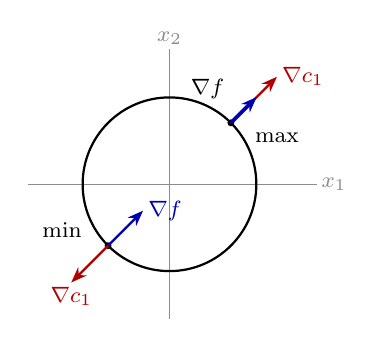
\begin{tikzpicture}[scale=0.78]
        \draw[black!45] (-2.3,0)--(2.4,0) node[lab,right]{$x_{1}$};
        \draw[black!45] (0,-2.2)--(0,2.2) node[lab,above]{$x_{2}$};
        \draw[thick] (0,0) circle (1.414);
        \fill (-1,-1) circle (1.6pt); \fill (1,1) circle (1.6pt);
        \draw[vec,blue!70!black] (-1,-1)--(-0.43,-0.43) node[lab,right]{$\gradf$};
        \draw[vec,red!70!black] (-1,-1)--(-1.6,-1.6) node[lab,below]{$\nabla c_{1}$};
        \draw[vec,red!70!black] (1,1)--(1.75,1.75) node[lab,right]{$\nabla c_{1}$};
        \draw[vec,blue!70!black,line width=1.4pt] (1,1)--(1.42,1.42);
        \node[lab] at (0.62,1.55) {$\gradf$};
        \node[lab] at (-1.75,-0.75) {min};
        \node[lab] at (1.75,0.75) {max};
      \end{tikzpicture}
    \end{column}
  \end{columns}
  \begin{center}\small\setlength\tabcolsep{8pt}
  \begin{tabular}{llll}
    \toprule
    $x$ & $\nabla c_{1}(x)$ & $\lambda_{1}$ & $f(x)$ \\
    \midrule
    $(-1,-1)^{T}$ & $(-2,-2)^{T}$ & $-\tfrac12$ & $-2$, the minimum on the circle \\
    $(1,1)^{T}$ & $(2,2)^{T}$ & $\tfrac12$ & $2$, the maximum on the circle \\
    \bottomrule
  \end{tabular}
  \end{center}
  The sign of $\lambda_{1}$ does not separate the two: with the constraint written as
  $2-x_{1}^{2}-x_{2}^{2}=0$, both signs change. \readbook{pp.~308--310.}
\end{frame}

\section{\S12.2 Tangent cone and LICQ}

\begin{frame}{Active set and linearized feasible directions}
  \begin{block}{Definition 12.1}
    The \textbf{active set} at a feasible $x$ is
    $\cA(x)=\cE\cup\{i\in\cI\mid c_{i}(x)=0\}$.\\
    Inequality constraint $i$ is \emph{active} if $c_{i}(x)=0$ and \emph{inactive} if $c_{i}(x)>0$.
  \end{block}
  \begin{block}{Definition 12.3}
    The set of \textbf{linearized feasible directions} at a feasible $x$ is
    \[ \cF(x)=\bigl\{d\ \bigm|\ d^{T}\nabla c_{i}(x)=0\ \ \forall i\in\cE,\quad
       d^{T}\nabla c_{i}(x)\ge 0\ \ \forall i\in\cA(x)\cap\cI\bigr\} . \]
  \end{block}
  \begin{itemize}\setlength\itemsep{0.3em}
    \item For an active constraint, $c_{i}(x+td)\approx c_{i}(x)+t\,\nabla c_{i}(x)^{T}d=t\,\nabla c_{i}(x)^{T}d$.
      $\cF(x)$ contains the directions $d$ along which this first-order model stays feasible.
    \item The KKT conditions contain only $\gradf$ and $\nabla c_{i}$. They see $\Omega$ only through $\cF(x)$.
  \end{itemize}
\end{frame}

\begin{frame}{The tangent cone}
  \textbf{Feasible sequence approaching $x$}: $z_{k}\in\Omega$ for all $k$ sufficiently large and $z_{k}\to x$.
  \begin{block}{Definition 12.2}
    The vector $d$ is a \textbf{tangent} to $\Omega$ at $x$ if there are a feasible sequence $\{z_{k}\}$
    approaching $x$ and a sequence of positive scalars $\{t_{k}\}$ with $t_{k}\to 0$ such that
    $\lim_{k\to\infty}(z_{k}-x)/t_{k}=d$ \eqn{12.29}.
    The set of all tangents to $\Omega$ at $\xs$ is the \textbf{tangent cone} $\TO(\xs)$.
  \end{block}
  \begin{itemize}\setlength\itemsep{0.4em}
    \item A tangent is a limiting direction along which one can approach $x$ while staying in $\Omega$.
    \item $\TO(x)$ is defined by the set $\Omega$ alone. The functions $c_{i}$ do not appear.
    \item It is a cone: if $d\in\TO(x)$ and $\alpha>0$, then $\alpha d\in\TO(x)$ (replace $t_{k}$ by $t_{k}/\alpha$).
  \end{itemize}
\end{frame}

\begin{frame}{Why both $\TO(x)$ and $\cF(x)$ are needed {\normalfont\small(Not in the book.)}}
  \begin{center}\small\setlength\tabcolsep{7pt}
  \renewcommand{\arraystretch}{1.15}
  \begin{tabular}{lll}
    \toprule
     & Tangent cone $\TO(x)$ & Linearized feasible directions $\cF(x)$ \\
    \midrule
    Defined by & the set $\Omega$ & the gradients $\nabla c_{i}(x)$ \\
    Describes $\Omega$ near $x$ & exactly, to first order & possibly with extra directions \\
    Can be computed & not in general & yes: linear equations and inequalities \\
    Used for & stating optimality & obtaining the multipliers $\lambda_{i}$ \\
    \bottomrule
  \end{tabular}
  \end{center}
  \begin{itemize}\setlength\itemsep{0.3em}
    \item Optimality is stated with $\TO$: at a local solution, $f$ cannot decrease to first order
      along any direction in $\TO(\xs)$.
    \item Multipliers come from $\cF$: a condition on $\cF(\xs)$ is a set of linear inequalities in $d$,
      and it can be converted into $\gradf(\xs)=\sum_{i}\lambda_{i}\nabla c_{i}(\xs)$.
    \item The argument starts in $\TO$ and continues in $\cF$. It is valid only if the two sets agree.
  \end{itemize}
\end{frame}

\begin{frame}{Example 12.4: the tangent cone of a circle}
  \begin{columns}[T,totalwidth=\textwidth]
    \begin{column}{0.64\textwidth}
      $\Omega$: the circle $x_{1}^{2}+x_{2}^{2}=2$ of (12.9). Point $x=(-\sqrt2,0)^{T}$.
      A feasible sequence approaching $x$:
      \[ z_{k}=\begin{bmatrix}-\sqrt{2-1/k^{2}}\\[0.1em] -1/k\end{bmatrix} . \tag{12.30} \]
    \end{column}
    \begin{column}{0.34\textwidth}
      \centering
      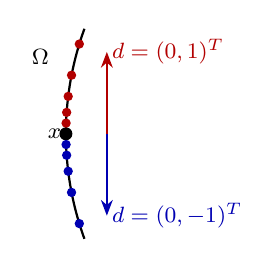
\begin{tikzpicture}[scale=1.3]
        \draw[thick] (160:3) arc (160:200:3);
        \fill (-3,0) circle (1.8pt) node[lab,left]{$x$};
        \foreach \a in {197,191,187,184,182}{\fill[blue!70!black] (\a:3) circle (1.3pt);}
        \foreach \a in {163,169,173,176,178}{\fill[red!70!black] (\a:3) circle (1.3pt);}
        \draw[vec,blue!70!black] (-2.6,0)--(-2.6,-0.8) node[lab,right]{$d=(0,-1)^{T}$};
        \draw[vec,red!70!black] (-2.6,0)--(-2.6,0.8) node[lab,right]{$d=(0,1)^{T}$};
        \node[lab] at (-3.25,0.75) {$\Omega$};
      \end{tikzpicture}
    \end{column}
  \end{columns}
  \begin{itemize}\setlength\itemsep{0.4em}
    \item With $t_{k}=\|z_{k}-x\|$, the limit of $(z_{k}-x)/t_{k}$ is $d=(0,-1)^{T}$. With
      $t_{k}=\|z_{k}-x\|/\alpha$, $\alpha>0$, it is $(0,-\alpha)^{T}$.
    \item The sequence with second component $+1/k$ approaches $x$ from the opposite side.
      Its tangents are $(0,\alpha)^{T}$, $\alpha>0$.
    \item The tangents at $x$ are the vectors whose first component is zero:
      $\TO(x)=\{(0,d_{2})^{T}\mid d_{2}\in\R\}$.
  \end{itemize}
  \readbook{pp.~317--318.}
\end{frame}

\begin{frame}{Example 12.5: tangent cone at an inequality boundary}
  \begin{columns}[T,totalwidth=\textwidth]
    \begin{column}{0.68\textwidth}
      $\Omega$: the disk $c_{1}(x)=2-x_{1}^{2}-x_{2}^{2}\ge 0$ of (12.18). Same $x=(-\sqrt2,0)^{T}$.\\[0.2em]
      The sequences of Example 12.4 are still feasible. There are more:
      for any $w=(w_{1},w_{2})^{T}$ with $w_{1}>0$, $z_{k}=x+(1/k)\,w$ is inside the disk
      for all $k$ sufficiently large. With $t_{k}=1/k$ its tangent is $w$.
    \end{column}
    \begin{column}{0.30\textwidth}
      \centering
      \begin{tikzpicture}[scale=0.82]
        \begin{scope}
          \clip (-3.05,-1.15) rectangle (-1.3,1.15);
          \fill[structure!25] (0,0) circle (3);
          \draw[thick] (0,0) circle (3);
        \end{scope}
        \draw[dashed] (-3,-1.15)--(-3,1.15);
        \fill (-3,0) circle (1.8pt) node[lab,left]{$x$};
        \draw[vec] (-3,0)--(-2.2,0.55) node[lab,right]{$w$};
        \draw[vec] (-3,0)--(-2.3,-0.5);
        \draw[vec] (-3,0)--(-3,0.9);
        \draw[vec] (-3,0)--(-3,-0.9);
        \node[lab] at (-1.75,-0.85) {$\Omega$};
      \end{tikzpicture}
    \end{column}
  \end{columns}
  \begin{itemize}\setlength\itemsep{0.3em}
    \item $\TO(x)=\{(w_{1},w_{2})^{T}\mid w_{1}\ge 0\}$: a half-space. It contains the tangent line and every
      direction pointing into $\Omega$.
    \item $\cF(x)$: $\nabla c_{1}(x)=(-2x_{1},-2x_{2})^{T}=(2\sqrt2,0)^{T}$. The condition for an active
      inequality is $\nabla c_{1}(x)^{T}d=2\sqrt2\,d_{1}\ge 0$. So $\cF(x)=\{d\mid d_{1}\ge 0\}=\TO(x)$.
    \item Circle (equality): tangent line. Disk (inequality): half-space.
      The inward directions are the source of the sign condition $\lambda_{i}\ge 0$.
  \end{itemize}
  \readbook{pp.~318--319.}
\end{frame}

\begin{frame}{$\cF(x)$ depends on how $\Omega$ is written: one circle, two descriptions}
  Same point $x=(-\sqrt2,0)^{T}$ as on the previous slide. Compute $\cF(x)$; $d=(d_{1},d_{2})^{T}$.

  \vspace{0.3em}
  \textbf{Description (12.9)}, $c_{1}(x)=x_{1}^{2}+x_{2}^{2}-2=0$.\\
  $\nabla c_{1}(x)=(2x_{1},2x_{2})^{T}=(-2\sqrt2,\,0)^{T}$ at this $x$.
  $\cF(x)$ is the set of $d$ with $\nabla c_{i}(x)^{T}d=0$ for every equality constraint (Definition 12.3). Here:
  \[ 0=\nabla c_{1}(x)^{T}d=(-2\sqrt2)\,d_{1}+0\cdot d_{2}=-2\sqrt2\,d_{1} . \]
  So $d_{1}=0$ and $d_{2}$ is free: $\cF(x)=\{(0,d_{2})^{T}\mid d_{2}\in\R\}=\TO(x)$.

  \vspace{0.2em}
  \textbf{Description (12.31)}, $c_{1}(x)=(x_{1}^{2}+x_{2}^{2}-2)^{2}=0$. The same circle $\Omega$.
  \[ \nabla c_{1}(x)=4(x_{1}^{2}+x_{2}^{2}-2)\begin{bmatrix}x_{1}\\x_{2}\end{bmatrix}=\begin{bmatrix}0\\0\end{bmatrix}
     \quad\text{at every feasible } x . \]
  The condition $0=\nabla c_{1}(x)^{T}d$ holds for all $d$: $\cF(x)=\R^{2}\ne\TO(x)$.

  $\TO(x)$ did not change. $\cF(x)$ changed with the algebraic description. \readbook{p.~318.}
\end{frame}

\begin{frame}{$\cF(x)$ can misrepresent $\Omega$: the constraints (12.32)}
  \begin{columns}[T,totalwidth=\textwidth]
    \begin{column}{0.72\textwidth}
      $c_{1}(x)=1-x_{1}^{2}-(x_{2}-1)^{2}\ge 0,\quad c_{2}(x)=-x_{2}\ge 0$ \eqn{12.32}.\\[0.3em]
      $c_{1}\ge 0$: the disk of radius 1 centered at $(0,1)^{T}$.\\
      $c_{2}\ge 0$: the half-plane $x_{2}\le 0$.\\
      The two sets have one common point: $\Omega=\{(0,0)^{T}\}$.
    \end{column}
    \begin{column}{0.26\textwidth}
      \centering
      \begin{tikzpicture}[scale=0.72]
        \fill[black!10] (-1.7,-0.6) rectangle (1.7,0);
        \fill[structure!30] (0,1) circle (1);
        \draw[thick] (0,1) circle (1);
        \draw[thick] (-1.7,0)--(1.7,0);
        \fill (0,0) circle (1.8pt);
        \node[lab] at (0,1) {$c_{1}\ge 0$};
        \node[lab] at (-0.9,-0.33) {$c_{2}\ge 0$};
        \node[lab,below] at (0.35,0) {$x$};
      \end{tikzpicture}
    \end{column}
  \end{columns}
  \begin{itemize}\setlength\itemsep{0.3em}
    \item $x=(0,0)^{T}$. Every feasible sequence has $z_{k}=x$ for large $k$, so $\TO(x)=\{(0,0)^{T}\}$.
    \item Both constraints are active. $\nabla c_{1}(x)=(-2x_{1},-2(x_{2}-1))^{T}=(0,2)^{T}$, $\nabla c_{2}(x)=(0,-1)^{T}$.
    \item $\cF(x)$ is the set of $d=(d_{1},d_{2})^{T}$ with $\nabla c_{i}(x)^{T}d\ge 0$ for every active inequality
      (Definition 12.3): $\nabla c_{1}(x)^{T}d=2d_{2}\ge 0$ and $\nabla c_{2}(x)^{T}d=-d_{2}\ge 0$.
    \item So $d_{2}=0$ and $d_{1}$ is free: $\cF(x)=\{(d_{1},0)^{T}\mid d_{1}\in\R\}$, the entire horizontal axis.
  \end{itemize}
  \readbook{pp.~319--320.}
\end{frame}

\begin{frame}{LICQ}
  A \textbf{constraint qualification} is a condition under which $\cF(x)$ is similar to $\TO(x)$.
  The LICQ makes the two sets identical (Lemma 12.2).
  \begin{block}{Definition 12.4 (LICQ)}
    Given the point $x$ and the active set $\cA(x)$, the \textbf{linear independence constraint
    qualification} holds if the set of active constraint gradients
    $\{\nabla c_{i}(x),\ i\in\cA(x)\}$ is linearly independent.
  \end{block}
  \vspace{0.2em}
  The three cases of the previous slides:
  \begin{center}\small\setlength\tabcolsep{8pt}
  \begin{tabular}{llll}
    \toprule
    Constraints & Active gradients at $x$ & LICQ & $\cF(x)=\TO(x)$? \\
    \midrule
    (12.9) & $(-2\sqrt2,0)^{T}$ & holds & yes \\
    (12.31) & $(0,0)^{T}$ & fails & no \\
    (12.32) & $(0,2)^{T}$, $(0,-1)^{T}$ & fails & no \\
    \bottomrule
  \end{tabular}
  \end{center}
\end{frame}

\begin{frame}{Lemma 12.2: what the LICQ gives}
  \begin{block}{Lemma 12.2}
    Let $\xs$ be a feasible point. The following two statements are true.
    \begin{itemize}
      \item[(i)] $\TO(\xs)\subset\cF(\xs)$.
      \item[(ii)] If the LICQ condition is satisfied at $\xs$, then $\cF(\xs)=\TO(\xs)$.
    \end{itemize}
  \end{block}
  \begin{itemize}\setlength\itemsep{0.35em}
    \item (i) is always true. Along a feasible sequence, $c_{i}(z_{k})=0$ (or $\ge 0$); a first-order
      Taylor expansion of $c_{i}$ gives $\nabla c_{i}(\xs)^{T}d=0$ (or $\ge 0$) for the tangent $d$.
    \item (ii): given $d\in\cF(\xs)$, a feasible sequence with limiting direction $d$ must be
      constructed. This is done with the implicit function theorem. Its Jacobian is nonsingular
      when the active gradients are linearly independent.
    \item $\cF(x)$ can be larger than $\TO(x)$, never smaller.
  \end{itemize}
  \readbook{proof of Lemma 12.2, pp.~323--325.}
\end{frame}

\section{\S12.3 First-order optimality conditions}

\begin{frame}{Theorem 12.1: the KKT conditions}
  Lagrangian for (12.1):\quad
  $\cL(x,\lambda)=f(x)-\sum_{i\in\cE\cup\cI}\lambda_{i}c_{i}(x)$ \eqn{12.33}.
  \begin{block}{Theorem 12.1 (First-Order Necessary Conditions)}
    \small Suppose that $\xs$ is a local solution of (12.1), that the functions $f$ and $c_{i}$ in (12.1) are
    continuously differentiable, and that the LICQ holds at $\xs$. Then there is a Lagrange multiplier
    vector $\ls$, with components $\ls_{i}$, $i\in\cE\cup\cI$, such that the following conditions are
    satisfied at $(\xs,\ls)$:
    \vspace{-0.8em}
    \begin{align}
      \nabla_{x}\cL(\xs,\ls) &= 0, \tag{12.34a}\\[-0.35em]
      c_{i}(\xs) &= 0\quad\text{for all } i\in\cE, \tag{12.34b}\\[-0.35em]
      c_{i}(\xs) &\ge 0\quad\text{for all } i\in\cI, \tag{12.34c}\\[-0.35em]
      \ls_{i} &\ge 0\quad\text{for all } i\in\cI, \tag{12.34d}\\[-0.35em]
      \ls_{i}\,c_{i}(\xs) &= 0\quad\text{for all } i\in\cE\cup\cI. \tag{12.34e}
    \end{align}
  \end{block}
  (12.34): the \textbf{Karush--Kuhn--Tucker (KKT) conditions}.
\end{frame}

\begin{frame}{Why the LICQ is assumed in Theorem 12.1}
  The proof has four steps. Only step 2 uses the LICQ.
  \begin{enumerate}\setlength\itemsep{0.3em}
    \item Theorem 12.3: if $\xs$ is a local solution, then $\gradf(\xs)^{T}d\ge 0$ for all $d\in\TO(\xs)$
      \eqn{12.43}. Reason: if $\gradf(\xs)^{T}d<0$ for a tangent $d$, then $f(z_{k})<f(\xs)$ along its
      feasible sequence for all large $k$.
    \item Lemma 12.2(ii), \alert{LICQ}: $\TO(\xs)=\cF(\xs)$. So $\gradf(\xs)^{T}d\ge 0$ for all $d\in\cF(\xs)$.
    \item Farkas' Lemma (Lemma 12.4): exactly one of the following is true.\\
      (a) $\gradf(\xs)=\sum_{i\in\cA(\xs)}\lambda_{i}\nabla c_{i}(\xs)$ with $\lambda_{i}\ge 0$ for
      $i\in\cA(\xs)\cap\cI$ \eqn{12.51}.\\
      (b) There is a $d\in\cF(\xs)$ with $\gradf(\xs)^{T}d<0$.\\
      Step 2 excludes (b), so (a) holds.
    \item Set $\ls_{i}=\lambda_{i}$ for $i\in\cA(\xs)$ and $\ls_{i}=0$ for inactive constraints \eqn{12.52}.
      This is (12.34).
  \end{enumerate}
  Step 1 is about $\TO$ (the set $\Omega$). Step 3 is about $\cF$ (the gradients). The LICQ connects them.
  \readbook{pp.~323--329.}
\end{frame}

\begin{frame}{Reading the KKT conditions}
  \begin{itemize}\setlength\itemsep{0.5em}
    \item (12.34e), complementarity: for each $i$, constraint $i$ is active or $\ls_{i}=0$, or both.
      Inactive inequalities have $\ls_{i}=0$, so (12.34a), $\nabla_{x}\cL(\xs,\ls)=0$, is
      \[ \gradf(\xs)=\sum_{i\in\cA(\xs)}\ls_{i}\nabla c_{i}(\xs) . \tag{12.35} \]
    \item Definition 12.5 (\textbf{strict complementarity}): exactly one of $\ls_{i}$ and $c_{i}(\xs)$
      is zero for each $i\in\cI$; that is, $\ls_{i}>0$ for each $i\in\cI\cap\cA(\xs)$.
    \item With the LICQ, $\ls$ is unique: the vectors $\nabla c_{i}(\xs)$, $i\in\cA(\xs)$, are linearly
      independent, so the coefficients in (12.35) are determined (Exercise 12.17).
    \item Without the LICQ, a local solution may have many multiplier vectors $\ls$, or none.
  \end{itemize}
  \readbook{pp.~320--322.}
\end{frame}

\section{\S12.5 Second-order conditions}

\begin{frame}{The critical cone}
  $f$, $c_{i}$ twice continuously differentiable; $(\xs,\ls)$ satisfies KKT; $w\in\cF(\xs)$.
  Multiply (12.35), $\gradf(\xs)=\sum_{i\in\cA(\xs)}\ls_{i}\nabla c_{i}(\xs)$, by $w^{T}$. The signs come from $w\in\cF(\xs)$:
  \[ w^{T}\gradf(\xs)=\sum_{i\in\cE}\ls_{i}\,\underbrace{w^{T}\nabla c_{i}(\xs)}_{=\,0}
     \ +\sum_{i\in\cA(\xs)\cap\cI}\underbrace{\ls_{i}}_{\ge\,0}\,\underbrace{w^{T}\nabla c_{i}(\xs)}_{\ge\,0}\ \ \ge 0 . \]
  \begin{itemize}\setlength\itemsep{0.4em}
    \item $w^{T}\gradf(\xs)>0$: $f$ increases along $w$ to first order. Nothing more to check.
    \item $w^{T}\gradf(\xs)=0$: first derivatives do not determine whether $f$ increases or decreases
      along $w$. This happens exactly when every term of the second sum is zero:
      $w^{T}\nabla c_{i}(\xs)=0$ for each active inequality with $\ls_{i}>0$.
  \end{itemize}
  \textbf{Critical cone}:
  \[ \cC(\xs,\ls)=\{w\in\cF(\xs)\mid\nabla c_{i}(\xs)^{T}w=0,\ \text{all } i\in\cA(\xs)\cap\cI \text{ with } \ls_{i}>0\} . \]
  \readbook{pp.~330--331.}
\end{frame}

\begin{frame}{Theorem 12.5: second-order necessary conditions}
  \begin{block}{Theorem 12.5 (Second-Order Necessary Conditions)}
    Suppose that $\xs$ is a local solution of (12.1) and that the LICQ condition is satisfied. Let $\ls$
    be the Lagrange multiplier vector for which the KKT conditions (12.34) are satisfied. Then
    \[ w^{T}\hessL(\xs,\ls)\,w\ge 0\quad\text{for all } w\in\cC(\xs,\ls) . \tag{12.57} \]
  \end{block}
  \begin{itemize}\setlength\itemsep{0.3em}
    \item The matrix is $\hessL=\hessf-\sum_{i}\ls_{i}\nabla^{2}c_{i}$, not $\hessf$.
      Only $w\in\cC$ is tested.
    \item Reason: along a feasible sequence with limiting direction $w\in\cC(\xs,\ls)$,
      $f(z_{k})=f(\xs)+\tfrac12 t_{k}^{2}\,w^{T}\hessL(\xs,\ls)\,w+o(t_{k}^{2})$ \eqn{12.64}. If $w^{T}\hessL\,w<0$,
      then $f(z_{k})<f(\xs)$ for large $k$. This contradicts that $\xs$ is a local solution.
      \readbook{pp.~332--333.}
  \end{itemize}
\end{frame}

\begin{frame}{Theorem 12.6: second-order sufficient conditions}
  \begin{block}{Theorem 12.6 (Second-Order Sufficient Conditions)}
    Suppose that for some feasible point $\xs\in\R^{n}$ there is a Lagrange multiplier vector $\ls$
    such that the KKT conditions (12.34) are satisfied. Suppose also that
    \[ w^{T}\hessL(\xs,\ls)\,w>0\quad\text{for all } w\in\cC(\xs,\ls),\ w\ne 0 . \tag{12.65} \]
    Then $\xs$ is a strict local solution for (12.1).
  \end{block}
  \begin{itemize}\setlength\itemsep{0.35em}
    \item No constraint qualification is required. In Theorem 12.5, $\ge$; here, $>$.
    \item Convex problem ($f$ convex, $-c_{i}$ convex for $i\in\cI$, $c_{i}$ affine for $i\in\cE$):
      $\hessL=\hessf-\sum_{i\in\cI}\ls_{i}\nabla^{2}c_{i}$ is positive semidefinite because $\ls_{i}\ge 0$.
      No second-order check is needed there. (Not in the book.)
  \end{itemize}
  \readbook{proof of Theorem 12.6, pp.~333--335.}
\end{frame}

\begin{frame}{Example 12.9: $\hessL$ can be indefinite at a solution}
  \[ \min\ -0.1(x_{1}-4)^{2}+x_{2}^{2}\quad\text{s.t.}\quad x_{1}^{2}+x_{2}^{2}-1\ge 0 \tag{12.72} \]
  \begin{itemize}\setlength\itemsep{0.3em}
    \item $\gradf(x)=(-0.2(x_{1}-4),\,2x_{2})^{T}$, $\nabla c_{1}(x)=(2x_{1},2x_{2})^{T}$.
      At $\xs=(1,0)^{T}$: $\gradf=(0.6,0)^{T}$, $\nabla c_{1}=(2,0)^{T}$, $c_{1}(\xs)=0$.
      $\gradf=\ls_{1}\nabla c_{1}$ with $\ls_{1}=0.3\ge 0$: KKT holds.
    \item $\ls_{1}>0$, so $\cC(\xs,\ls)$ requires $\nabla c_{1}(\xs)^{T}w=2w_{1}=0$:
      $\cC(\xs,\ls)=\{(0,w_{2})^{T}\mid w_{2}\in\R\}$.
    \item $\hessL(x,\lambda)=\hessf-\lambda_{1}\nabla^{2}c_{1}=\mathrm{diag}(-0.2-2\lambda_{1},\ 2-2\lambda_{1})$ \eqn{12.73b}.
      For $w\in\cC(\xs,\ls)$: $w^{T}\hessL(\xs,\ls)\,w=1.4\,w_{2}^{2}>0$.
    \item $\hessL(\xs,\ls)=\mathrm{diag}(-0.8,\,1.4)$ is indefinite. Its negative-curvature direction
      $(1,0)^{T}$ is not in $\cC(\xs,\ls)$. So $(1,0)^{T}$ is a strict local solution.
  \end{itemize}
  {\small (The book prints $-0.4$ on p.~336; (12.73b) gives $-0.8$. Same conclusion.)}
\end{frame}

\begin{frame}{Example 12.9: the picture {\normalfont\small(Figure not in the book.)}}
  \begin{columns}[T,totalwidth=\textwidth]
    \begin{column}{0.54\textwidth}
      \centering
      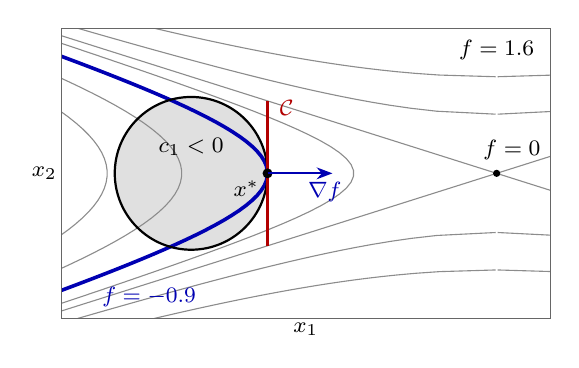
\begin{tikzpicture}[x=0.97cm,y=0.97cm]
        \begin{scope}
          \clip (-1.7,-1.9) rectangle (4.7,1.9);
          \fill[black!12] (0,0) circle (1);
          % contours f = c, left branch x1 = 4 - sqrt(10(t^2 - c)), c < 0
          \foreach \c in {-2.6,-1.7,-0.35}{
            \draw[black!45] plot[domain=-1.9:1.9,samples=50,variable=\t] ({4-sqrt(10*(\t*\t-(\c)))},{\t});}
          % f = 0: two lines through the saddle point (4,0)
          \draw[black!45] (4,0)--({4-sqrt(10)*1.9},1.9) (4,0)--({4-sqrt(10)*1.9},-1.9);
          \draw[black!45] (4,0)--({4+sqrt(10)*1.9},1.9) (4,0)--({4+sqrt(10)*1.9},-1.9);
          % f = c > 0
          \foreach \c in {0.6,1.6}{
            \draw[black!45] plot[domain={sqrt(\c)}:1.9,samples=30,variable=\t] ({4-sqrt(abs(10*(\t*\t-\c)))},{\t});
            \draw[black!45] plot[domain={sqrt(\c)}:1.9,samples=30,variable=\t] ({4+sqrt(abs(10*(\t*\t-\c)))},{\t});
            \draw[black!45] plot[domain={sqrt(\c)}:1.9,samples=30,variable=\t] ({4-sqrt(abs(10*(\t*\t-\c)))},{-\t});
            \draw[black!45] plot[domain={sqrt(\c)}:1.9,samples=30,variable=\t] ({4+sqrt(abs(10*(\t*\t-\c)))},{-\t});}
          % the contour through x*: f = -0.9
          \draw[blue!70!black,line width=1.3pt] plot[domain=-1.9:1.9,samples=60,variable=\t] ({4-sqrt(10*(\t*\t+0.9))},{\t});
          \draw[thick] (0,0) circle (1);
          % critical cone
          \draw[red!70!black,line width=1.3pt] (1,-0.95)--(1,0.95);
        \end{scope}
        \draw[black!60] (-1.7,-1.9) rectangle (4.7,1.9);
        \fill (1,0) circle (1.8pt);
        \fill (4,0) circle (1.3pt);
        \draw[vec,blue!70!black] (1,0)--(1.85,0);
        \node[lab,blue!70!black] at (1.75,-0.25) {$\gradf$};
        \node[lab] at (0.72,-0.2) {$\xs$};
        \node[lab,red!70!black] at (1.25,0.85) {$\cC$};
        \node[lab] at (0,0.35) {$c_{1}<0$};
        \node[lab,blue!70!black] at (-0.55,-1.62) {$f=-0.9$};
        \node[lab] at (4.0,1.62) {$f=1.6$};
        \node[lab] at (4.2,0.3) {$f=0$};
        \node[lab,below] at (1.5,-1.9) {$x_{1}$};
        \node[lab,left] at (-1.7,0) {$x_{2}$};
      \end{tikzpicture}
    \end{column}
    \begin{column}{0.44\textwidth}
      \vspace{0.6em}
      Feasible set: outside the unit circle.\\[0.3em]
      Gray: contours of $f$.\\[0.3em]
      {\color{blue!70!black}Blue}: the contour $f=-0.9$ through $\xs=(1,0)^{T}$.
      To its right, $f>-0.9$.\\[0.3em]
      {\color{red!70!black}Red}: the critical cone $\cC(\xs,\ls)$.
    \end{column}
  \end{columns}
  \begin{itemize}\setlength\itemsep{0.2em}
    \item Near $\xs$ the circle is to the right of the blue contour: nearby feasible points have a larger $f$.
      On the circle, $f=-0.9+0.7\,\theta^{2}+\cdots$, and $0.7=\tfrac12 w^{T}\hessL\,w$ for $w=(0,1)^{T}\in\cC$.
    \item $\hessf=\mathrm{diag}(-0.2,2)$ has negative curvature along $x_{1}$, but $(1,0)^{T}\notin\cC$.
      Not global: $f\to-\infty$ as $x_{1}\to\infty$.
  \end{itemize}
\end{frame}


\section{\S12.8 and \S12.9: sensitivity and duality}

\begin{frame}{Lagrange multipliers and sensitivity}
  Perturb an active constraint $i$: require $c_{i}(x)\ge-\epsilon\|\nabla c_{i}(\xs)\|$ instead of
  $c_{i}(x)\ge 0$. Suppose $\epsilon$ is small enough that the perturbed solution $\xs(\epsilon)$ has
  the same active set and the multipliers are not much affected. Then
  \[ \frac{d f(\xs(\epsilon))}{d\epsilon}=-\ls_{i}\,\|\nabla c_{i}(\xs)\| . \tag{12.80} \]
  \begin{itemize}\setlength\itemsep{0.25em}
    \item The derivation is informal. It can be made rigorous with strict complementarity and
      second-order conditions.
    \item Definition 12.8: $c_{i}$ is \textbf{strongly active} (\textbf{binding}) if $i\in\cA(\xs)$ and
      $\ls_{i}>0$ for some $\ls$ satisfying the KKT conditions; \textbf{weakly active} if $i\in\cA(\xs)$ and
      $\ls_{i}=0$ for all such $\ls$.
    \item Replacing $c_{i}$ by $10c_{i}$ gives $\ls_{i}/10$ and $10\nabla c_{i}(\xs)$:
      (12.80) does not change.
  \end{itemize}
  \readbook{pp.~341--343.}
\end{frame}

\begin{frame}{Duality: the dual objective and the dual problem}
  No equality constraints; $c(x)=(c_{1}(x),\dots,c_{m}(x))^{T}$; $\cL(x,\lambda)=f(x)-\lambda^{T}c(x)$.
  \[ \min_{x\in\R^{n}} f(x)\quad\text{subject to}\quad c(x)\ge 0 . \tag{12.81} \]
  \textbf{Dual objective function} \eqn{12.82} and \textbf{dual problem} \eqn{12.84}:
  \[ q(\lambda)\stackrel{\rm def}{=}\inf_{x}\cL(x,\lambda),\qquad\qquad
     \max_{\lambda\in\R^{m}} q(\lambda)\quad\text{subject to}\quad\lambda\ge 0 . \]
  \begin{itemize}\setlength\itemsep{0.3em}
    \item Theorem 12.10: $q$ is concave and its domain $D=\{\lambda\mid q(\lambda)>-\infty\}$ is convex.
    \item Theorem 12.11 (weak duality): $q(\bar\lambda)\le f(\bar x)$ for any feasible $\bar x$ and any
      $\bar\lambda\ge 0$.
    \item Theorem 12.12: if $\bar x$ solves (12.81) and $f$, $-c_{i}$ are convex and differentiable at $\bar x$,
      then any $\bar\lambda$ for which $(\bar x,\bar\lambda)$ satisfies the KKT conditions solves (12.84).
    \item Wolfe dual \eqn{12.88}:\ \
      $\max_{x,\lambda}\ \cL(x,\lambda)$\ \ subject to\ \ $\nabla_{x}\cL(x,\lambda)=0,\ \lambda\ge 0$.
  \end{itemize}
  Theorems 12.10 and 12.11 assume no convexity. \readbook{pp.~343--348.}
\end{frame}

\section{Chapter 12: summary and homework}

\begin{frame}{Chapter 12 in one table}
  \begin{center}\small\setlength\tabcolsep{5pt}
  \renewcommand{\arraystretch}{1.2}
  \begin{tabular}{lll}
    \toprule
    Result & Assumption at $\xs$ & Statement \\
    \midrule
    Lemma 12.2 & (i) none;\ \ (ii) LICQ & (i) $\TO\subset\cF$;\ \ (ii) $\TO=\cF$ \\
    Theorem 12.3 & local solution & $\gradf^{T}d\ge 0$ for all $d\in\TO$ \\
    Theorem 12.1 & local solution, LICQ & KKT conditions (12.34) \\
    Theorem 12.5 & local solution, LICQ & $w^{T}\hessL\,w\ge 0$ for all $w\in\cC$ \\
    Theorem 12.6 & KKT and (12.65) & strict local solution \\
    (12.80) & same active set (informal) & $df(\xs(\epsilon))/d\epsilon=-\ls_{i}\|\nabla c_{i}\|$ \\
    Theorems 12.10, 12.11 & none & $q$ concave; $q(\bar\lambda)\le f(\bar x)$ \\
    Theorem 12.12 & $f$, $-c_{i}$ convex & a KKT multiplier solves the dual \\
    \bottomrule
  \end{tabular}
  \end{center}
  \begin{itemize}\setlength\itemsep{0.3em}
    \item Necessary conditions (Theorems 12.1, 12.5) assume the LICQ.
    \item The sufficient condition (Theorem 12.6) assumes no constraint qualification.
  \end{itemize}
\end{frame}

\begin{frame}{Homework {\normalfont\small(problems 2, 3, 5 are not in the book)}}
  \begin{enumerate}\setlength\itemsep{0.35em}
    \item Exercise 12.14: $H=\{x\in\R^{n}\mid a^{T}x+\alpha\ge 0\}$ with given $a\in\R^{n}$, $\alpha\in\R$.
      Find the point in $H$ with the smallest Euclidean norm, using the KKT conditions.
    \item Constraints (12.32), $\xs=(0,0)^{T}$, $f(x)=x_{1}$. (a) Show that $\xs$ is the solution.
      (b) Show that no $\lambda$ satisfies $\gradf(\xs)=\sum_{i}\lambda_{i}\nabla c_{i}(\xs)$. (c) Which of the four steps in the proof of
      Theorem 12.1 fails, and for which $d$?
    \item $f(x)=x_{1}+x_{2}$. (a) Constraint $2-x_{1}^{2}-x_{2}^{2}\ge 0$: which KKT condition does
      $(1,1)^{T}$ violate? (b) Constraint $x_{1}^{2}+x_{2}^{2}-2\ge 0$: show that $(1,1)^{T}$ satisfies the KKT
      conditions. Is it a local solution?
    \item Exercise 12.19: $\min\,-2x_{1}+x_{2}$ s.t.\ $(1-x_{1})^{3}-x_{2}\ge 0$,
      $x_{2}+0.25x_{1}^{2}-1\ge 0$, at $\xs=(0,1)^{T}$. Parts (a)--(d).
    \item $\min\ 0.5(x_{1}^{2}+x_{2}^{2})$ s.t.\ $x_{1}-1\ge-\epsilon$. Find $\xs(\epsilon)$ and
      $f(\xs(\epsilon))$ by hand, and check (12.80) with $\ls_{1}=1$.
  \end{enumerate}
\end{frame}

\end{document}
